\documentclass[12pt, a4paper, fleqn]{memoir}%makeidx

%******************************************************************************
% STYLE
%******************************************************************************
%******************************************************************************
% PACKAGES
%******************************************************************************
\usepackage{graphicx}
\usepackage{epsfig}
\usepackage{amsmath}
\usepackage{amssymb}
\usepackage{amsthm}
\usepackage{booktabs}
\usepackage{stmaryrd}
\usepackage{url}
\usepackage[figuresright]{rotating}
\usepackage{listings}
\usepackage{algorithm}
\usepackage{algpseudocode}
\usepackage{pifont}
\usepackage{ifsym}
\usepackage{relsize}
\usepackage[ansinew]{inputenc}
%\usepackage{dingbat}
\usepackage{hhline}
\usepackage{booktabs}
%\usepackage{xtab}
%\usepackage[margin=10pt,font={small,sf},labelfont=bf]{caption}
%\usepackage{tabularx}
%\usepackage{longtable}
%\usepackage{multirow}
\usepackage{color}
\usepackage{colortbl}
\usepackage{fancyvrb}
\usepackage{rotating}
\usepackage{makeidx}
\usepackage{MnSymbol}
\usepackage{textcomp}
%******************************************************************************
% INDEX GENERATION
%******************************************************************************
\makeindex

%******************************************************************************
% HYPEREF/ALGORITHM FIX
%******************************************************************************
\newcommand{\theHalgorithm}{\arabic{algorithm}}

% Konfiguration von hyperref
%\hypersetup{pdftex=true, colorlinks=true, breaklinks=true,
%   linkcolor=schwarz, menucolor=schwarz, pagecolor=schwarz, urlcolor=schwarz, citecolor=schwarz}

%******************************************************************************
% NUMBERING
%******************************************************************************
\numberwithin{algorithm}{chapter}
\numberwithin{figure}{chapter}

%******************************************************************************
% PAGE NUMBER IN BIBLIOGRAPHY
%******************************************************************************
\usepackage{citeref}
\renewcommand{\bibitempages}[1]{\newblock {\scriptsize [\mbox{cited at p.\ }#1]}}

%******************************************************************************
% PDF HYPERLINKS
%******************************************************************************
\ifpdf
  \pdfcompresslevel=9
        \usepackage[plainpages=false,pdfpagelabels,bookmarksnumbered,%
        colorlinks=true,%
        linkcolor=blue,%
        citecolor=blue,%
        filecolor=blue,%
        pagecolor=blue,%
        urlcolor=blue,%
        pdftex,
        unicode]{hyperref} 
    \input supp-mis.tex
    \input supp-pdf.tex
    \pdfimageresolution=600
    \usepackage{thumbpdf} 
\else
    \usepackage{hyperref}
\fi
\usepackage{memhfixc}

%******************************************************************************
% PAGE LAYOUT
%******************************************************************************
%\settypeblocksize{*}{32pc}{1.618}
%\setlrmargins{*}{1.47in}{*}
%\setulmargins{*}{*}{1.3}
%\setheadfoot{\onelineskip}{2\onelineskip}
%\setheaderspaces{*}{2\onelineskip}{*}
%\def\baselinestretch{1.1}
%\checkandfixthelayout



\newcolumntype{H}[1]{>{\columncolor[gray]{0.90}}p{#1}}
\newcolumntype{I}[1]{>{\centering\columncolor[gray]{0.90}}p{#1}}
\newcolumntype{q}[1]{>{\centering}p{#1}}
\renewcommand{\arraystretch}{1.25}
%******************************************************************************
% CHAPTER AND SECTION STYLE
%******************************************************************************
\makechapterstyle{mychapterstyle}{%
    \renewcommand{\chapnamefont}{\LARGE\sffamily\bfseries}%
    \renewcommand{\chapnumfont}{\LARGE\sffamily\bfseries}%
    \renewcommand{\chaptitlefont}{\Huge\sffamily\bfseries}%
    \renewcommand{\printchaptertitle}[1]{%
        \chaptitlefont\hrule height 0.5pt \vspace{1em}%
        {##1}\vspace{1em}\hrule height 0.5pt%
        }%
    \renewcommand{\printchapternum}{%
        \chapnumfont\thechapter%
        }%
}
\chapterstyle{mychapterstyle}
\setsecheadstyle{\Large\sffamily\bfseries}
\setsubsecheadstyle{\large\sffamily\bfseries}
\setsubsubsecheadstyle{\normalfont\sffamily\bfseries}
\setparaheadstyle{\normalfont\sffamily}
\makeevenhead{headings}{\thepage}{}{\small\slshape\leftmark}
\makeoddhead{headings}{\small\slshape\rightmark}{}{\thepage}

%******************************************************************************
% TABLE OF CONTENTS STYLE
%******************************************************************************
\settocdepth{subsection}
\setsecnumdepth{subsection}
\maxsecnumdepth{subsection}
\settocdepth{subsection}
\maxtocdepth{subsection}

%******************************************************************************
% COMMANDS FOR EPIGRAPHS
%******************************************************************************
\setlength{\epigraphwidth}{0.57\textwidth}
\setlength{\epigraphrule}{0pt}
\setlength{\beforeepigraphskip}{1\baselineskip}
\setlength{\afterepigraphskip}{2\baselineskip}
\newcommand{\epitext}{\sffamily\itshape}
\newcommand{\epiauthor}{\sffamily\scshape ---~}
\newcommand{\epititle}{\sffamily\itshape}
\newcommand{\epidate}{\sffamily\scshape}
\newcommand{\episkip}{\medskip}
\newcommand{\myepigraph}[4]{%
	\epigraph{\epitext #1\episkip}{\epiauthor #2\\\epititle #3 \epidate(#4)}\noindent}


%******************************************************************************
% FOOTNOTE STYLE
%******************************************************************************
\renewcommand{\thefootnote}{\fnsymbol{footnote}}

%******************************************************************************
% COLORS
%******************************************************************************
\usepackage{color}
\definecolor{greenyellow}   {cmyk}{0.15, 0   , 0.69, 0   }
\definecolor{yellow}        {cmyk}{0   , 0   , 1   , 0   }
\definecolor{goldenrod}     {cmyk}{0   , 0.10, 0.84, 0   }
\definecolor{dandelion}     {cmyk}{0   , 0.29, 0.84, 0   }
\definecolor{apricot}       {cmyk}{0   , 0.32, 0.52, 0   }
\definecolor{peach}         {cmyk}{0   , 0.50, 0.70, 0   }
\definecolor{melon}         {cmyk}{0   , 0.46, 0.50, 0   }
\definecolor{yelloworange}  {cmyk}{0   , 0.42, 1   , 0   }
\definecolor{orange}        {cmyk}{0   , 0.61, 0.87, 0   }
\definecolor{burntorange}   {cmyk}{0   , 0.51, 1   , 0   }
\definecolor{bittersweet}   {cmyk}{0   , 0.75, 1   , 0.24}
\definecolor{redorange}     {cmyk}{0   , 0.77, 0.87, 0   }
\definecolor{mahogany}      {cmyk}{0   , 0.85, 0.87, 0.35}
\definecolor{maroon}        {cmyk}{0   , 0.87, 0.68, 0.32}
\definecolor{brickred}      {cmyk}{0   , 0.89, 0.94, 0.28}
\definecolor{red}           {cmyk}{0   , 1   , 1   , 0   }
\definecolor{orangered}     {cmyk}{0   , 1   , 0.50, 0   }
\definecolor{rubinered}     {cmyk}{0   , 1   , 0.13, 0   }
\definecolor{wildstrawberry}{cmyk}{0   , 0.96, 0.39, 0   }
\definecolor{salmon}        {cmyk}{0   , 0.53, 0.38, 0   }
\definecolor{carnationpink} {cmyk}{0   , 0.63, 0   , 0   }
\definecolor{magenta}       {cmyk}{0   , 1   , 0   , 0   }
\definecolor{violetred}     {cmyk}{0   , 0.81, 0   , 0   }
\definecolor{rhodamine}     {cmyk}{0   , 0.82, 0   , 0   }
\definecolor{mulberry}      {cmyk}{0.34, 0.90, 0   , 0.02}
\definecolor{redviolet}     {cmyk}{0.07, 0.90, 0   , 0.34}
\definecolor{fuchsia}       {cmyk}{0.47, 0.91, 0   , 0.08}
\definecolor{lavender}      {cmyk}{0   , 0.48, 0   , 0   }
\definecolor{thistle}       {cmyk}{0.12, 0.59, 0   , 0   }
\definecolor{orchid}        {cmyk}{0.32, 0.64, 0   , 0   }
\definecolor{darkorchid}    {cmyk}{0.40, 0.80, 0.20, 0   }
\definecolor{purple}        {cmyk}{0.45, 0.86, 0   , 0   }
\definecolor{plum}          {cmyk}{0.50, 1   , 0   , 0   }
\definecolor{violet}        {cmyk}{0.79, 0.88, 0   , 0   }
\definecolor{royalpurple}   {cmyk}{0.75, 0.90, 0   , 0   }
\definecolor{blueviolet}    {cmyk}{0.86, 0.91, 0   , 0.04}
\definecolor{periwinkle}    {cmyk}{0.57, 0.55, 0   , 0   }
\definecolor{cadetblue}     {cmyk}{0.62, 0.57, 0.23, 0   }
\definecolor{cornflowerblue}{cmyk}{0.65, 0.13, 0   , 0   }
\definecolor{midnightblue}  {cmyk}{0.98, 0.13, 0   , 0.43}
\definecolor{navyblue}      {cmyk}{0.94, 0.54, 0   , 0   }
\definecolor{royalblue}     {cmyk}{1   , 0.50, 0   , 0   }
\definecolor{blue}          {cmyk}{1   , 1   , 0   , 0   }
\definecolor{cerulean}      {cmyk}{0.94, 0.11, 0   , 0   }
\definecolor{cyan}          {cmyk}{1   , 0   , 0   , 0   }
\definecolor{processblue}   {cmyk}{0.96, 0   , 0   , 0   }
\definecolor{skyblue}       {cmyk}{0.62, 0   , 0.12, 0   }
\definecolor{turquoise}     {cmyk}{0.85, 0   , 0.20, 0   }
\definecolor{tealblue}      {cmyk}{0.86, 0   , 0.34, 0.02}
\definecolor{aquamarine}    {cmyk}{0.82, 0   , 0.30, 0   }
\definecolor{bluegreen}     {cmyk}{0.85, 0   , 0.33, 0   }
\definecolor{emerald}       {cmyk}{1   , 0   , 0.50, 0   }
\definecolor{junglegreen}   {cmyk}{0.99, 0   , 0.52, 0   }
\definecolor{seagreen}      {cmyk}{0.69, 0   , 0.50, 0   }
\definecolor{green}         {cmyk}{1   , 0   , 1   , 0   }
\definecolor{forestgreen}   {cmyk}{0.91, 0   , 0.88, 0.12}
\definecolor{pinegreen}     {cmyk}{0.92, 0   , 0.59, 0.25}
\definecolor{limegreen}     {cmyk}{0.50, 0   , 1   , 0   }
\definecolor{yellowgreen}   {cmyk}{0.44, 0   , 0.74, 0   }
\definecolor{springgreen}   {cmyk}{0.26, 0   , 0.76, 0   }
\definecolor{olivegreen}    {cmyk}{0.64, 0   , 0.95, 0.40}
\definecolor{rawsienna}     {cmyk}{0   , 0.72, 1   , 0.45}
\definecolor{sepia}         {cmyk}{0   , 0.83, 1   , 0.70}
\definecolor{brown}         {cmyk}{0   , 0.81, 1   , 0.60}
\definecolor{tan}           {cmyk}{0.14, 0.42, 0.56, 0   }
\definecolor{gray}          {cmyk}{0   , 0   , 0   , 0.50}
\definecolor{black}         {cmyk}{0   , 0   , 0   , 1   }
\definecolor{white}         {cmyk}{0   , 0   , 0   , 0   } 
\definecolor{cell}          {cmyk}{0   , 0   , 0   , 0.25} 
\definecolor{stahlblau}		  {rgb} {0.2,0.56,0.84}
\definecolor{graurot}       {rgb} {0.62,0.15,0.15}
\definecolor{schwarz}       {rgb} {0.0,0.0,0.0}


%******************************************************************************
% BEGIN DOCUMENT
%******************************************************************************
\begin{document}

%******************************************************************************
% FRONT MATTER
%******************************************************************************
\frontmatter

%******************************************************************************
% EMPTY PAGE
%******************************************************************************
\pagestyle{empty}
This is actually the first page of the thesis and will be discarded after the print out. This is done because 
the title page has to be an even page. The memoir style package used by this template makes different indentations 
for odd and even pages which is usally done for better readability.  
\clearpage

%******************************************************************************
% TITLE PAGE
%******************************************************************************
\pagestyle{empty}
\rmfamily
\noindent
\begin{center}
University of Augsburg\\
Faculty of Applied Computer Science\\
Department of Computer Science\\
Bachelor's Program in Computer Science\\
\end{center}
\begin{figure}[h]
\centering

\includegraphics[width=0.25\textwidth]{logo.png}
\end{figure}
\vfill\vfill
\begin{center}
\Large
Bachelor's Thesis\\
\end{center}
\vspace{2.0em}
\begin{center}
\Large
\LARGE Engagement Detection\\ \vspace{10pt} 
\Large Inferring conversational engagement from verbak and nonverbal behaviour
\end{center}
\vspace{2.0em}
\begin{center}
    \normalsize
    submitted by\\
    \large
    Amr Abdelraouf\\
    \normalsize
    on 31.7.2014
\end{center}
\vspace{2.0em}
\begin{center}
    \normalsize
    Supervisor:\\ 
    Prof. Dr. Elisabeth Andr\'{e} aus Augsburg
\end{center}
\begin{center}
    \normalsize
    Adviser:\\
    MSc. Tobias Baur
\end{center}
\begin{center}
    \normalsize
    Reviewers:\\
    Prof. Dr. Elisabeth Andr\'{e}\\
\end{center}
\cleardoublepage

%******************************************************************************
% ABSTRACT
%******************************************************************************
\chapter*{Abstract}
Interview skills are of utmost important for a person's career and personal image. Furthermore it is an essential matter to exhude conversational engagement in an interview to give the impression of confidence and attentiveness. This thesis aims to track the engagment level of an interviewee in a mock interview situation. It tracks the verbal and nonverbal behaviour of the interviewee with respect to the ongoing context of the interview. The gathered engagement data can be further used to assess the interviewee's performance.

%******************************************************************************
% STATEMENT & DECLARATION
%******************************************************************************
\chapter*{Statement and Declaration of Consent}
\vfill
\subsubsection*{\LARGE Statement}
Hereby I confirm that this thesis is my own work and that I have documented all sources used.
\vfill
\begin{flushleft}
Amr Abdelraouf
\end{flushleft}  
\begin{flushright}
Augsburg, 3.7.2014 
\end{flushright}
\vfill
\vfill
\subsubsection*{\LARGE Declaration of Consent}
Herewith I agree that my thesis will be made available through the library of the Computer Science Department.
\vfill
\begin{flushleft}
Amr Abdelraouf
\end{flushleft}  
\begin{flushright}
Augsburg, 3.7.2014 
\end{flushright}
\vfill

%******************************************************************************
% TABLE OF CONTENTS
%******************************************************************************
\cleardoublepage
\rmfamily
\normalfont
\pagenumbering{roman}
\pagestyle{headings}
\tableofcontents


%******************************************************************************
% MAIN MATTER
%******************************************************************************
\mainmatter

%##########################################################
\chapter{Introduction}
\label{chap:Introduction}

\section{Motivation}
\label{sec:Motivation}
This thesis was proposed to help measure the engagement of an interviewee in a job interview situation. Through a simple mock interview the performance of the interviewee will be assessed. One of the most important attributes of that performance is whether or not the interviwee is engaged with and attentive to the interviewer. A simple playback of the interview coupled with the measurment of the engagement level will easily highlight the ups and downs of his/her demonstration in the mock interview.

\section{Objectives}
\label{sec:Objectives}
This thesis aims to measure the engagement levels of an interviewee through verbal and non verbal behaviour of said interview. It studies the conversational interaction with the interviewer, the responses to certain commands and behaviour during certain segments of the interview.

\section{Outline}
\label{sec:Outline}
This thesis will first discuss the theoretical background and the information gathered on this subject. It will go into the details of the work previously done. Next it will describe the setup of it's mock interview from both the interviewer and the intervieweee's perspectives.

In the following section details of constitution and software workings of this thesis will be covered. First it will describe the general structure of the pipeline. Then it will describe how the inputs are processed from a bottom up approach; starting with raw sensor data and working up level by level to demonstrate how the engagement is calculated.

%##########################################################
\chapter{Theoretical Background}
\label{chap:TheoreticalBackground}

\section{Previous Work}
\label{sec:PreviousWork}

[EXTENSIVE EXPLANATION ABOUT THE PREVIOUSLY READ PAPERS. CONCENTRATE MOST ON THE RICH PAPER]

\section{Setup}
\label{sec:Section}

\subsection{Subject}
\label{subsec:Subject}
The subject of our experiment is the interviewee in our mock interview. As shown in figure \ref{fig:setup_img} the subject is seated aproximately 70 cm from a screen. A number of sensors are then set up to capture the needed inputs. Namely a Microsoft Kinect, an SMI Eyetracker and a microphone.

\subsection{Agent}
\label{subsec:Agent}
There are two main softwares used to simulate the virtual interview environment. First there is Charamel. Charamel is responsible for creating the interviewers (or agents) and their surrounding environment. The scene used for this thesis consists of two virtual characters, namely Curtis and Gloria. They stand behind a desk to mimic an office interview. On the left lies a white board that is used as an object in our environment. The setting is demonstrated in figure \ref{fig:agents_img}.

The second software used is Scenemaker. Scenemaker is responsible for sending the agents actions to perform. The program consists of a state machine, each state containing a command to be executed by the agents accordingly. These commands include ordering the agents to utter a certain sentence, stop and wait for the subject to reply, perform a certain hand gesture, and so on and so forth.

\begin{figure}[h]
    \centering
    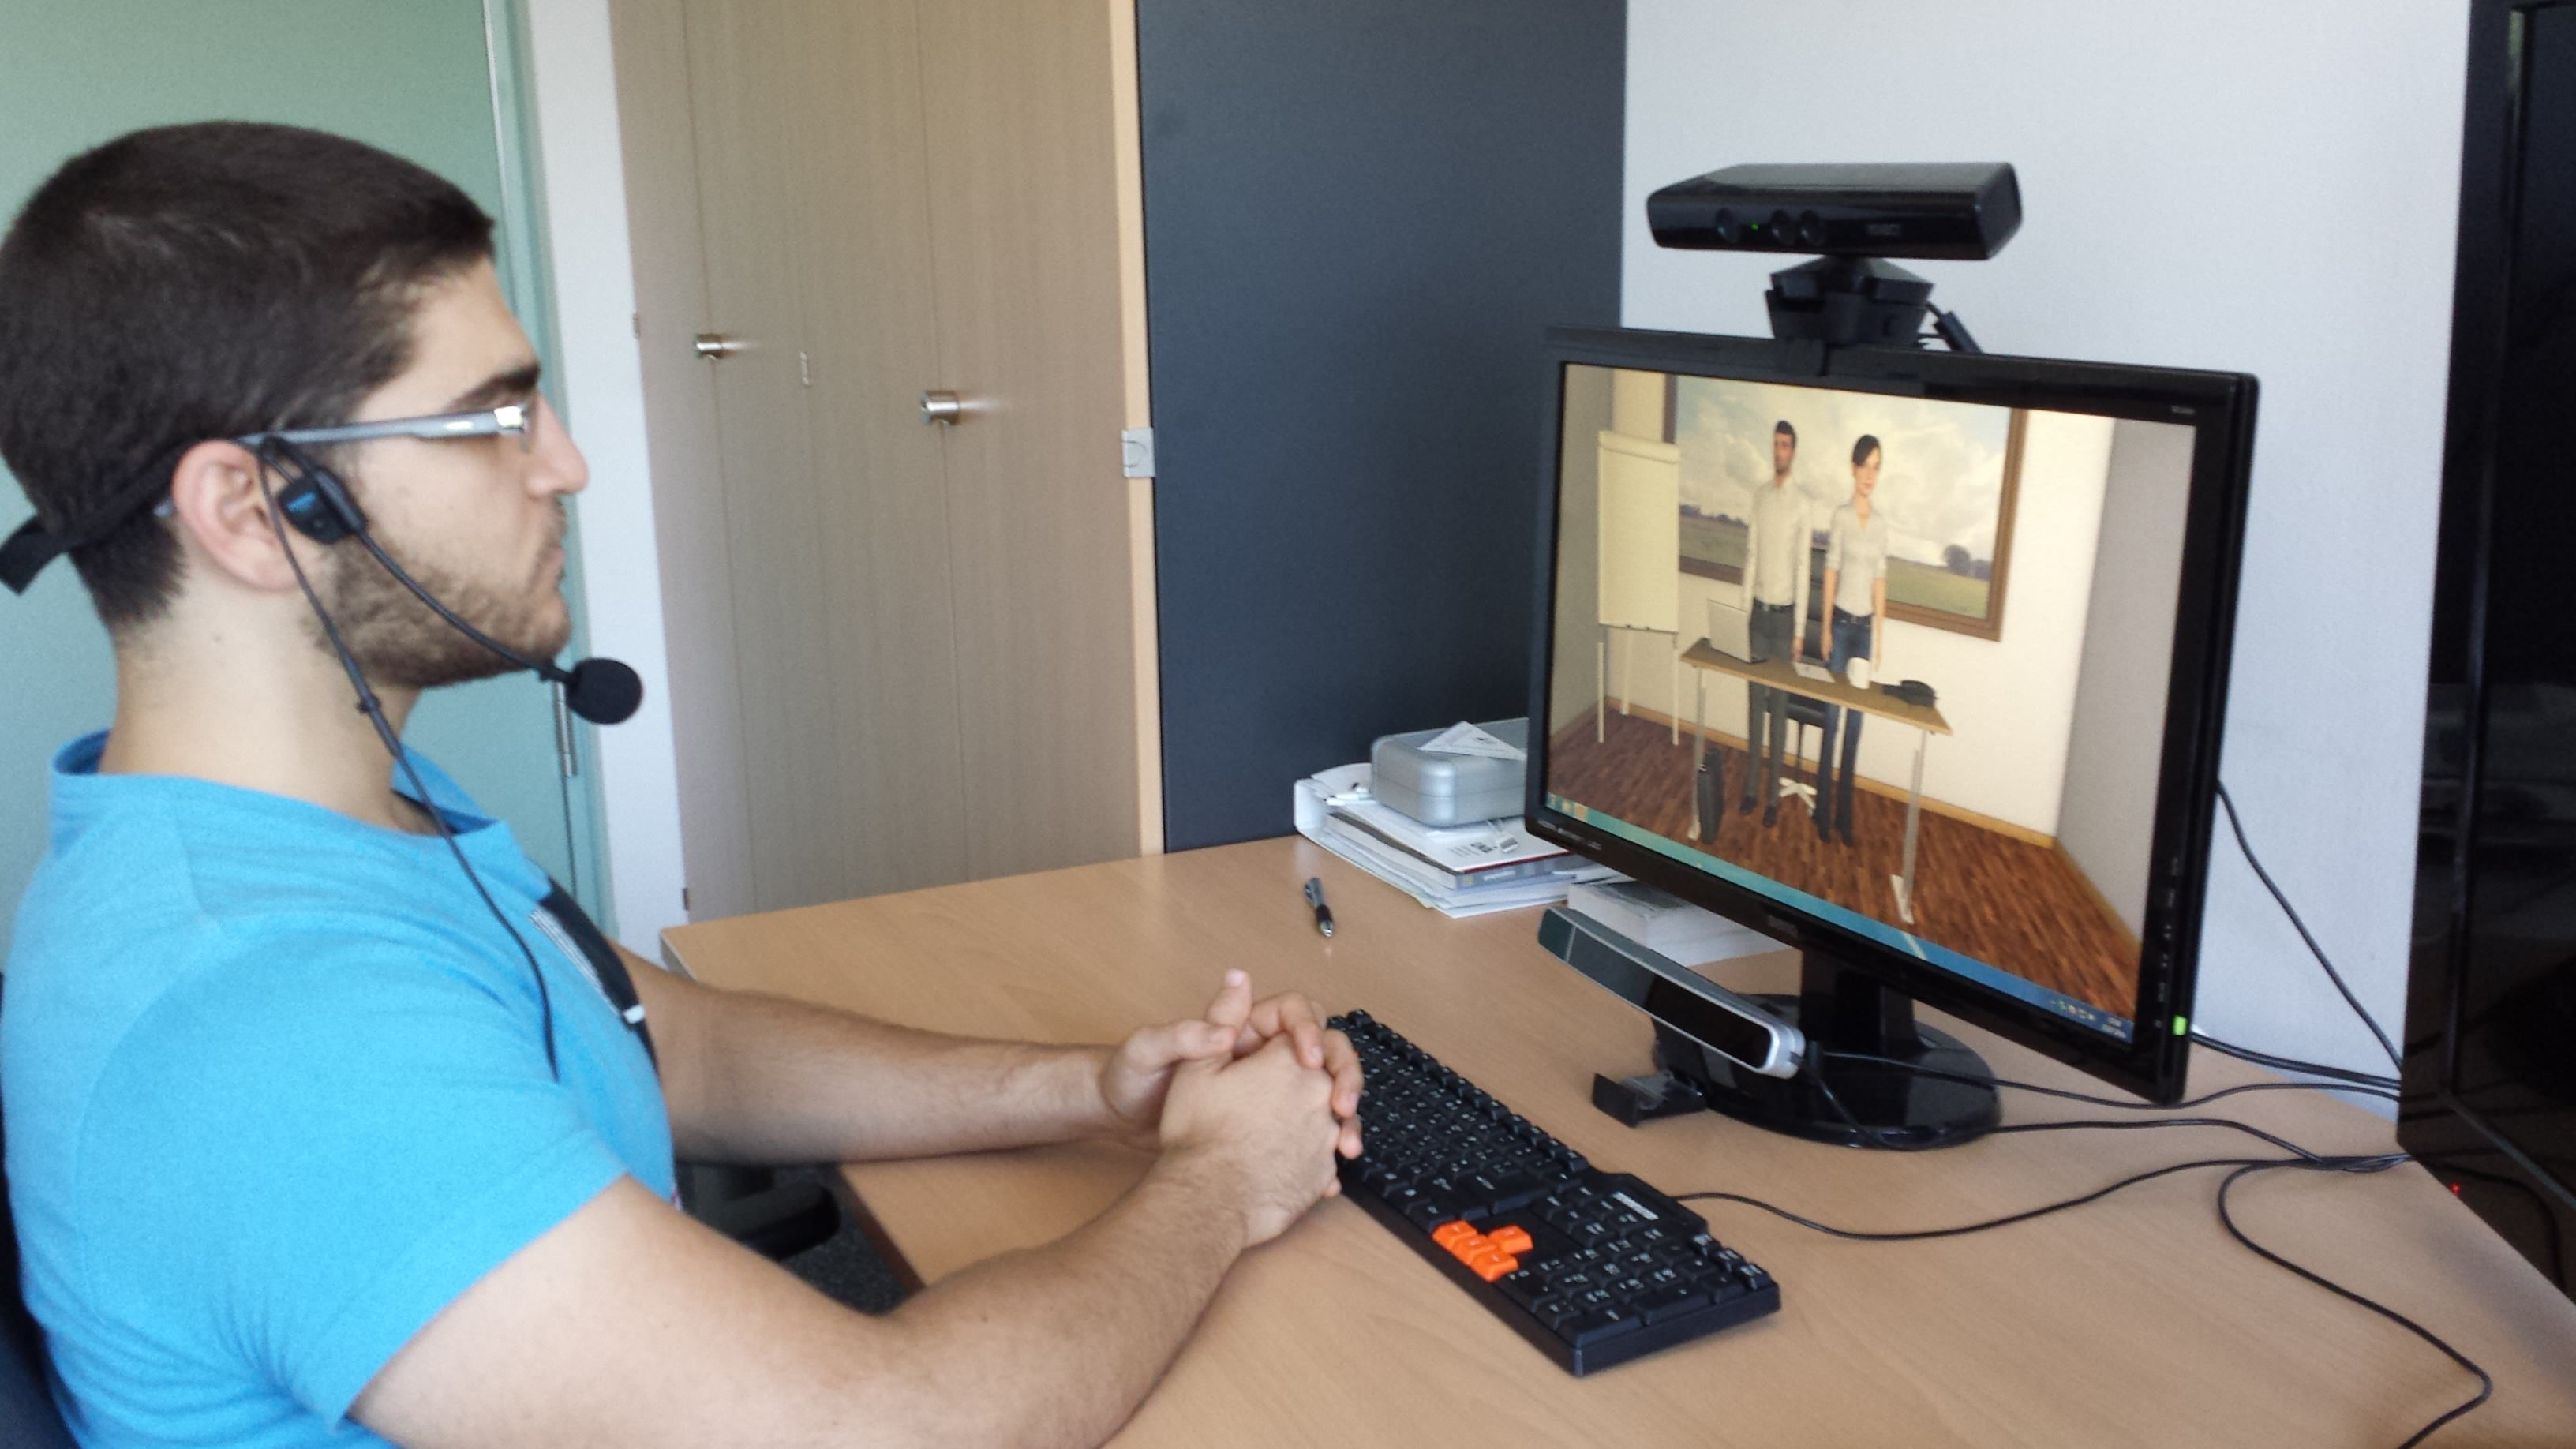
\includegraphics[width=1\textwidth]{setup}
    \caption{Interview setup}
    \label{fig:setup_img}
\end{figure}

\begin{figure}[h]
    \centering
    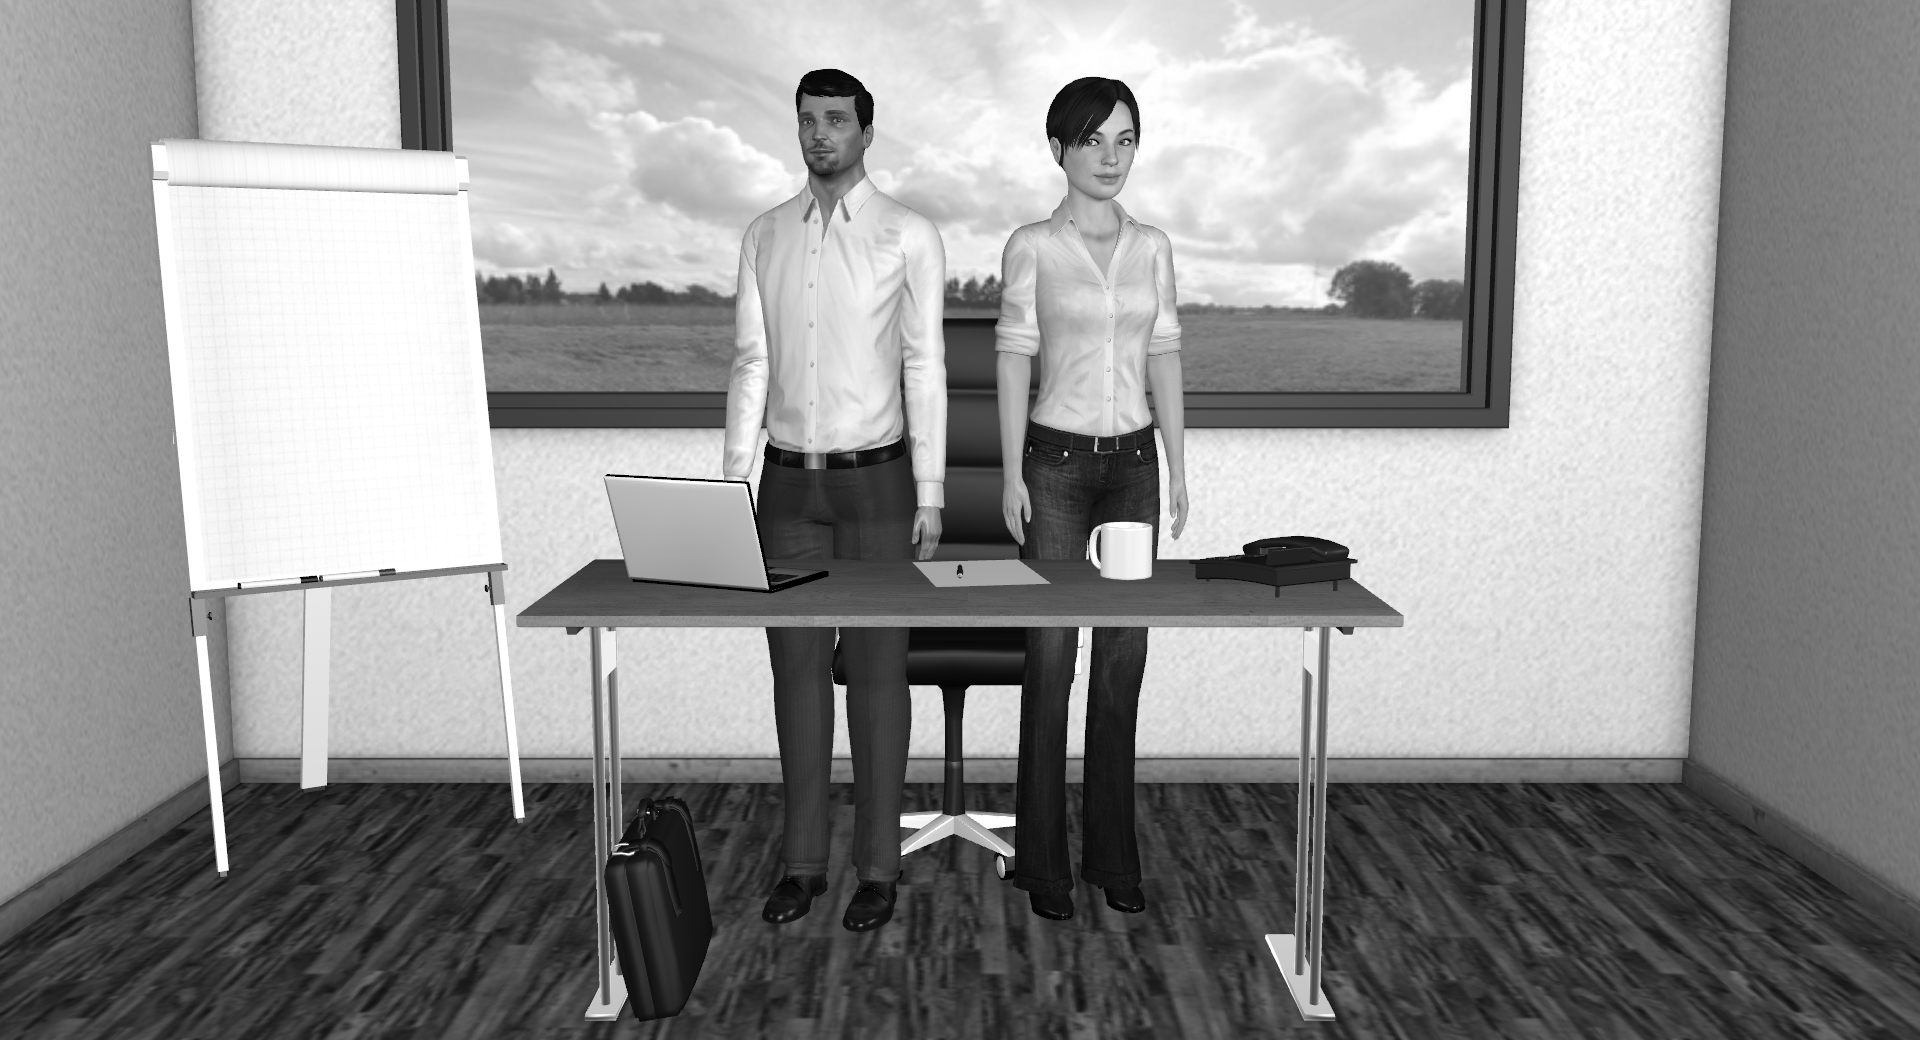
\includegraphics[width=1\textwidth]{agents}
    \caption{Virtual environment}
    \label{fig:agents_img}
\end{figure}

%%##########################################################
\chapter{Events}
\label{chap:Events}
Events are the backbone of the software workings of this thesis. Raw sensor data are converted to events that can be further processed in the software's pipeline. Furthermore external software send events to our own software over a network. These events can be displayed by themselves as output or can be used as inputs to trigger other events.

\section{Event Structure}
Events are constructs of several attributes:

\begin{description}
  \item[Time] The clock signature of when the event was triggered.
  \item[Duration] The time duration of the event.
  \item[Ptr] (Pointer) Meta data about the event.
  \item[Type] Indicates the nature of the meta data wrapped by the event.
  \item[State] A boolean flag to indicate whether the event is starting or ending.
\end{description}

In the software's pipeline events are measuerd every time cycle. A cycle of 500 ms is used.

\section{Sensors}
\label{sec:Sensors}

\subsection{Microsoft Kinect}
[MORE DESCRIPTION]

Kinect sensors are used to track the skeletal movements of a subject. However in this module we are mainly interested in the movement of the subject's head. Kinect is used to detect the prepetual displacement of the subject's head which indicates that s/he is nodding. This triggers an event called \textit{HeadNod}. HeadNod is an event measured and outputed every 500 ms and its pointer contains a value from 0 to 1 which represents the probability that the subject is nodding his/her head.

\subsection{SMI Eyetracker}
[MORE DESCRIPTION]

The SMI Eyetracker is used to pinpoint where the subject is currently looking. Since we are dealing with a virtual agent on a screen we consider the top left corner of the screen as the (0,0) coordinate. Displacement of the subject's gaze point to the right alters the x coordinate and to the bottom affects the y coordinate.

The software defines two main rectangular areas on the screen. First is the area of the Agent's face. Second is the area of the board that is present in the environment.

When the subject's gaze point falls on the area defined for the agent's face it triggers an event called \textit{SubjectFacialGaze}. SubjectFacialGaze's pointer contains a value of either 0 or 1 indicating whether or not the subject is looking at the agent's face. When the gaze enters the facial area SubjectFacialGaze is triggered with the value 1 indicating that it has started and when the gaze leaves the facial area it is triggered with the value 0 indicating that it is complete.

If the subject's gaze falls in the area of the board the event \textit{SubjectObjectGaze} is triggered. Similar to SubjectFacialGaze, the event carries a value of either 0 or 1 indicating whether or not the subject is looking at the board. The event is prompted with pointer value 1 when the subject starts looking at the object, and triggered again with 0 when the subject directs his/her gaze away.

\subsection{Microphone}
A microphone is used to record the verbal utterances produced by the subject. When the microphone detects a voice the event \textit{vad} (which is short for Voice Activity Duration) is fired. When the voice is first detected the event's pointer carries a value of 1. When the voice activity ends the same event is triggered but with value 0 to indicate that the event is complete.

\section{Scenemaker}
\label{sec:Scenemaker}
As mentioned before in subsection \ref{subsec:Agent} Scenemaker is the software used to send commands to the virtual agents. Scenemaker is also responsible for sending the events that are triggered to represent the agents' behaviour to our software's pipeline. The events can be subcategorized into two main parts: Gaze and speech.

\subsection{Gaze}
Firstly we are concerned with where the agent is looking. When the script commands the agent to looks at the subject in front of the screen the event \textit{AgentFacialGaze} is triggered. Similar to the subject's gaze events the event pointer holds the value 1 when the agent starts looking at the subject and holds the value 0 when the agent looks away from the subject's face.

Furthermore when the agent is commanded to look at the board, the event \textit{AgentObjectGaze} is triggered with a pointer value 1 or 0 indicating that the agent has started or stopped looking at the board.

\subsection{Speech}
The agent utters the sentences that are written in the affiliated script. When the agent starts reading a sentence the event \textit{AgentSpeech} is triggered with a pointer value of 1. When the agent finishes reading that sentence AgentSpeech is triggered with a pointer value of 0.

%%##########################################################
\chapter{Main Modules}
\label{chap:MainModules}
So to review our events, we have:

\begin{itemize}
  \item HeadNod
  \item SubjectFacialGaze
  \item SubjectObjectGaze
  \item vad
  \item AgentFacialGaze
  \item AgentObjectGaze
  \item AgentSpeech
\end{itemize}

Those events will be used as inputs for our four main modules.

\section{Mutual Facial Gaze}
\label{sec:MutualFacialGaze}
Mutual Facial Gaze is defined as the eye contact between the subject and the agent. It is necessary for the subject to direct his/her gaze at the agent's face when being addressed. The event \textit{MutualFacialGaze} is triggered with a pointer value 1 (indicating that it started) when both SubjectFacialGaze and AgentFacialGaze are ongoing. When either of the two input events are triggered with the value 0 (event ends) the event MutualFacialGaze is also ends and therefore is triggered with pointer value 0.

\section{Directed Gaze}
\label{sec:DirectedGaze}
Directed Gaze occurs when the agent points or looks at a certain object and then the subject follows. In our environment the white board acts as the object. The event \textit{DirectedGaze} is triggered with pointer value 1 when both SubjectObjectGaze and AgentObjectGaze are ongoing. And triggered again with pointer value 0 when one of the two input events ends.

\section{Adjacency Pair}
\label{sec:AdjacencyPair}
Adjacency Pairs are usually defined as a speech utterance which is provoked by a previous speech utterance. For instance the answer to a question is an adjacency pair. This thesis did not go into the the semantics of natural language processing. The inputs where when the agent started and stopped speaking, and when the subject started and stopped speaking. Naturally we redefined the meaning of adjacency pairs to match our inputs.

This thesis defines adjacency pairs as a verbal statement uttered by the subject within a window of two seconds after the agent has finished speaking. It is assumed that any statement spoken by the subject shortly after the agent finishes is provoked by the agent's previous sentence. The \textit{AdjacencyPair} start event is fired when a vad start event is detected within 2 seconds of an AgentSpeech end event. An AdjacencyPair end event is prompted as soon as said vad event ends.

\section{Backchanneling}
\label{sec:Backchanneling}
Backchanneling is the small responses given by the subject during the time where the agent is speaking. These responses indicate that the subject is following what the agent is saying. [CHECK HOW THE RICH PAPER DESCRIBES IT]

Here we introduce the concept of a \textit{Backchanneling Pulse}. Since backchanneling has a very short duration that usually lasts only one event cycle which is not enough time to influence the bayesian network. So instead when a backchanneling event is provoked it is outputed on 5 consecutive event cycles with pointer value 1, 0.75, 0.5, 0.25 and 0 respectively, as shown in figure \ref{fig:bcp_img}.

\begin{figure}[h]
    \centering
    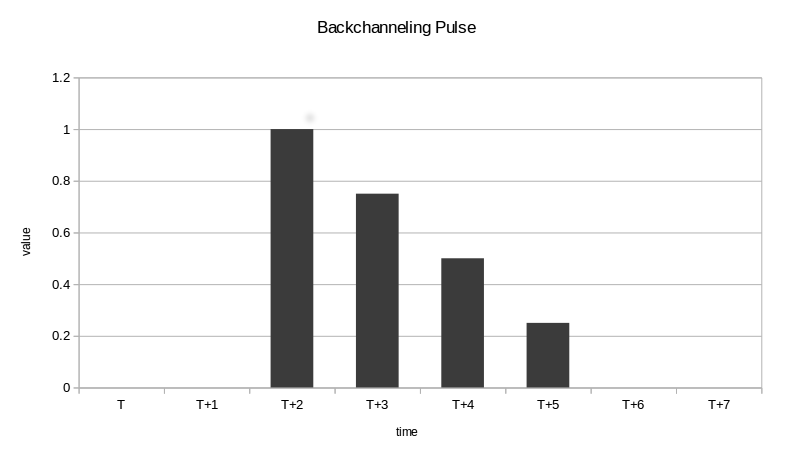
\includegraphics[width=1\textwidth]{bcp}
    \caption{Backchanneling event triggered at T+2}
    \label{fig:bcp_img}
\end{figure}

A BCPulse can be triggered by two different ways. It can be prompted when a HeadNod is detected during AgentSpeech. Or it can be set off when a vad event with a duration less than 2 seconds is detected during an AgentSpeech.

%%##########################################################
\chapter{Bayesian Network}
\label{chap:BayesianNetwork}
[ASK TOBY ABOUT HOW MUCH YOU CAN WRITE ABOUT THE BAYESIAN NETWORK. MINIMALLY JUST TALK ABOUT HOW THE ENGAGEMENT IS CALCULATED FEL AER]

%%##########################################################
\chapter{Summary}
\label{Summary}
[EXPLAIN THE GENERAL STRUCTURE AGAIN IN MORE DETAIL THIS TIME. ADD IMAGE SHOWING YOUR SO CALLED BOTTOM UP APPROACH]
%******************************************************************************
% BIBLIOGRAPHY
%******************************************************************************
\bibliographystyle{plain}
{\small\bibliography{master}}

%******************************************************************************
% APPENDIX
%******************************************************************************
%\appendix
%\appendixpage*
%\chapter{First Appendix}

%******************************************************************************
% BACK MATTER
%******************************************************************************
\backmatter

%******************************************************************************
% LIST OF SYMBOLS
%******************************************************************************
%\normalfont
%\clearpage
%\chapter[List of Symbols and Abbreviations]{List of Symbols and Abbreviations}
%\begin{center}
%\small
%\begin{longtable}{lp{3.0in}c}
%\toprule
%\multicolumn{1}{c}{Abbreviation} & \multicolumn{1}{c}{Description}\\ \midrule\addlinespace[2pt] \endhead
%\bottomrule\endfoot
%XML & E\textbf{X}tensible \textbf{M}arkup \textbf{L}anguage \\
%XSD & \textbf{X}ML-\textbf{S}chema-\textbf{D}efinition \\
%SFXML & \textbf{S}cene\textbf{F}low E\textbf{X}tensible \textbf{M}arkup \textbf{L}anguage \\
%SFTXL & \textbf{S}cene\textbf{F}low \textbf{T}extual E\textbf{X}pression \textbf{L}anguage \\
%SCXML & \textbf{S}tate\textbf{C}hart E\textbf{X}tensible \textbf{M}arkup \textbf{L}anguage \\
%DOM & \textbf{D}ocument \textbf{O}bject \textbf{M}odel \\
%LR & \textbf{L}eft to \textbf{R}ightmost derivation \\
%LALR & \textbf{L}ook\textbf{A}head LR\\
%NPC & \textbf{N}on-\textbf{P}erson-\textbf{C}haracter\\
%ABL & \textbf{A} \textbf{B}ehavior \textbf{L}anguage\\
%\end{longtable}
%\end{center}

%******************************************************************************
% LIST OF FIGURES
%******************************************************************************
\normalfont
\clearpage
\listoffigures

%******************************************************************************
% LIST OF TABLES
%******************************************************************************
\normalfont
\clearpage
\listoftables

%******************************************************************************
% LIST OF ALGORITHMS
%******************************************************************************
%\normalfont
\clearpage
\listofalgorithms

%******************************************************************************
% END DOCUMENT
%******************************************************************************
\end{document}
